\documentclass[border=10pt]{standalone}

\usepackage{tikz}
\usepackage{tikzsymbols}
\usetikzlibrary{calc,patterns,shapes.geometric}

\def\centerarc[#1](#2)(#3:#4:#5){\draw[#1] ($(#2)+({#5*cos(#3)},{#5*sin(#3)})$) arc (#3:#4:#5);}

\begin{document}
	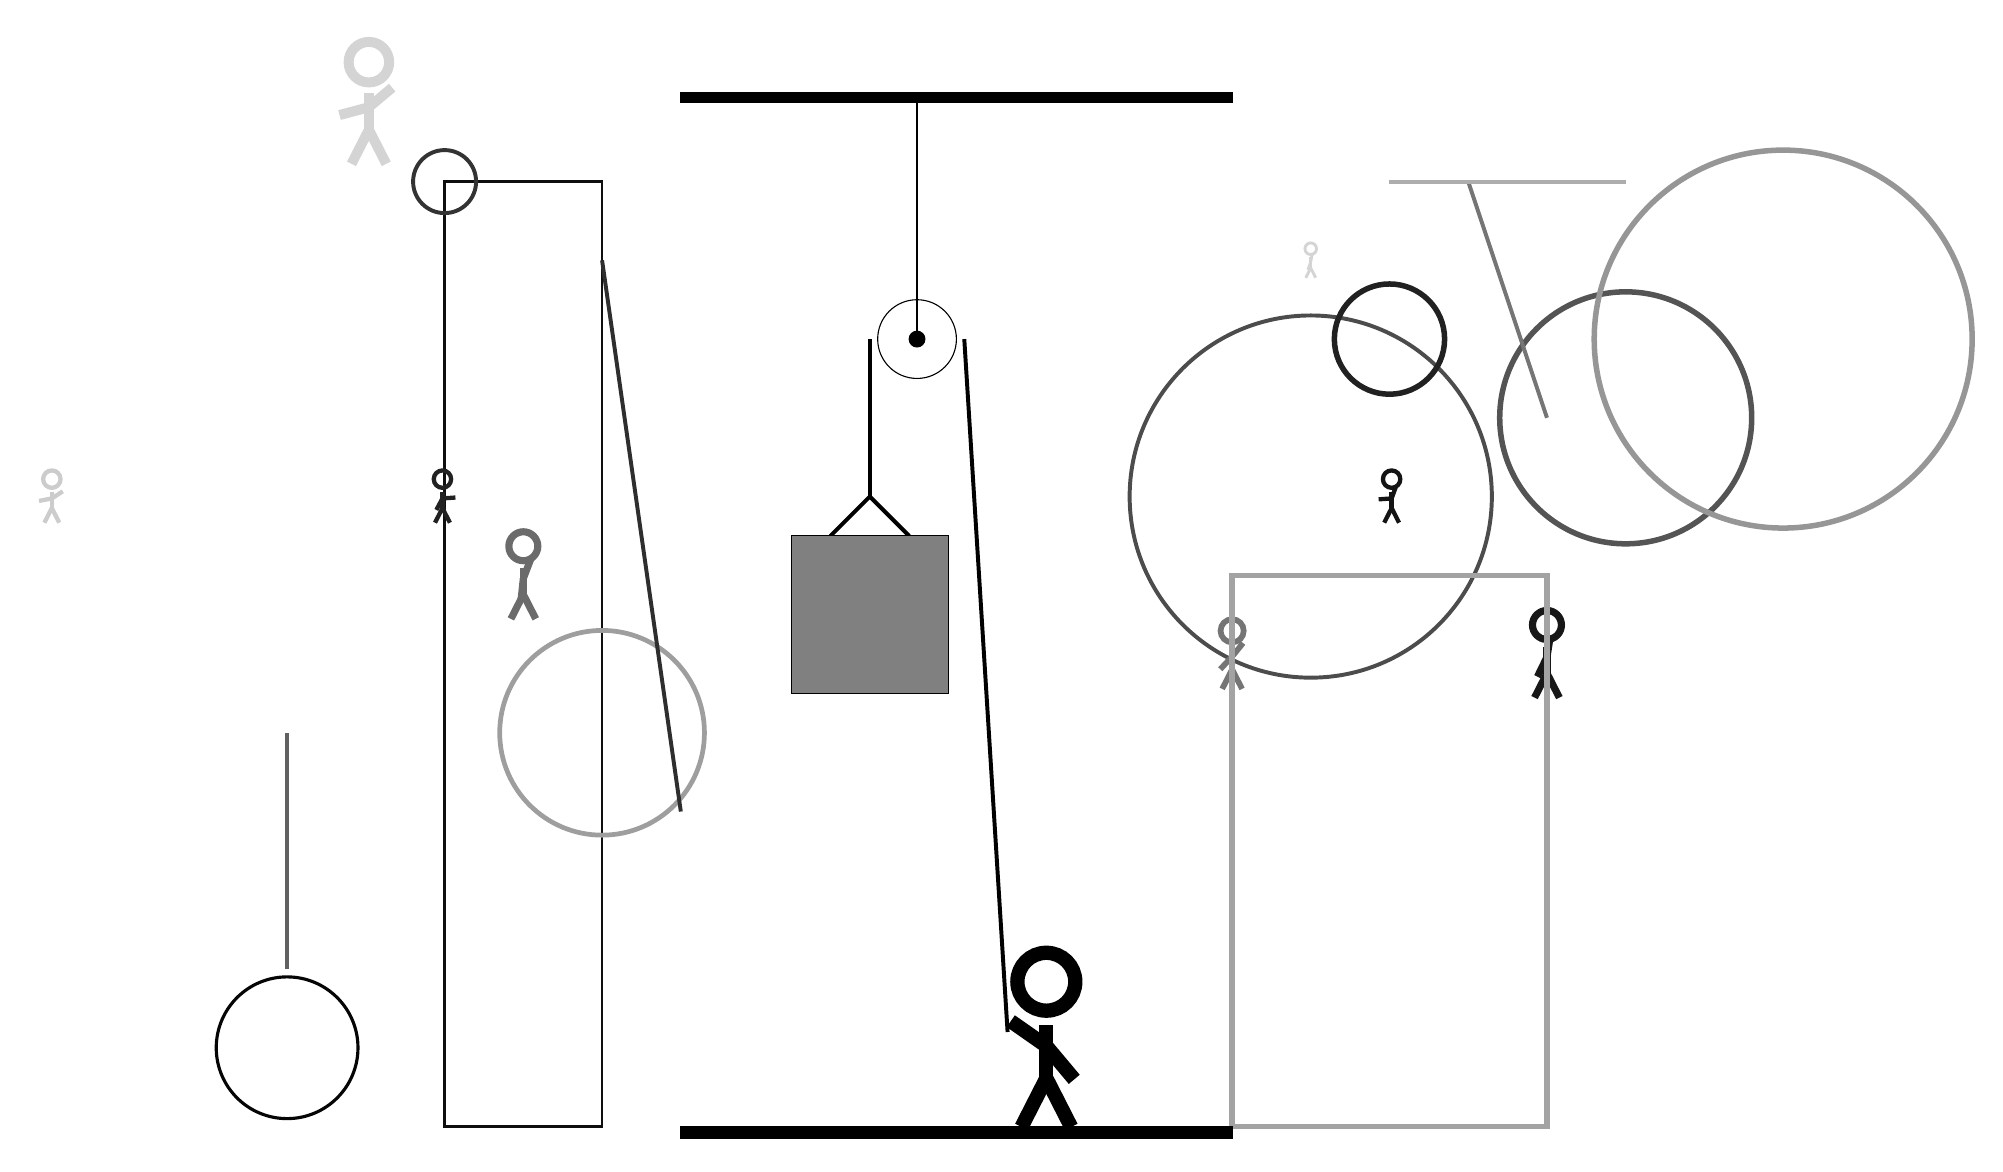
\begin{tikzpicture}
		%%%%% START %%%%%
		
		\draw[fill=black] (-2, 10) rectangle (5, 10.125);
		
		\draw (1, 7) circle (0.5);
		\draw[fill=black] (1, 7) circle (0.1);
		\draw (1, 10) -- (1, 7);
		
		\draw[line width=0.5mm] (-0.1, 4.5) -- (0.4, 5.0) -- (0.9, 4.5);
		\draw[fill=black!50] (-0.6, 4.5) rectangle (1.4, 2.5);
		
		\draw[line width=0.5mm] (0.4, 7) -- (0.4, 5.0);
		\centerarc[line width=0.5mm](1, 7)(0:180:0.6);
		\draw[line width=0.5mm](1.6, 7) -- (2.15, -1.8);
		
		\draw[line width=0.3mm, color=black!94] (-3, 9) rectangle (-5, -3);
		
		\draw[line width=0.5mm, color=black!62](-7, -1) -- (-7, 2);
		\node[line width=0.7mm, color=black!87] at (-5, 5) {\Strichmaxerl[3][62][4]};
		\draw [line width=0.5mm, color=black!80](-5, 9) circle (0.4);
		\node[line width=0.7mm, color=black!20] at (-10, 5) {\Strichmaxerl[3][11][33]};
		\draw [line width=0.7mm, color=black!67](10, 6) circle (1.6);
		\draw [line width=0.4mm, color=black!98](-7, -2) circle (0.9);
		
		\draw [line width=0.6mm, color=black!38](-3, 2) circle (1.3);
		\draw [line width=0.5mm, color=black!70](6, 5) circle (2.3);
		\node[line width=0.7mm, color=black!58] at (-4, 4) {\Strichmaxerl[5][84][69]};
		\node[line width=0.7mm, color=black!92] at (7, 5) {\Strichmaxerl[3][4][70]};
		\node[line width=0.2mm, color=black!54] at (5, 3) {\Strichmaxerl[4][47][51]};
		\node[line width=0.4mm, color=black!91] at (9, 3) {\Strichmaxerl[5][64][81]};
		\node[line width=0.7mm, color=black!17] at (-6, 10) {\Strichmaxerl[7][15][40]};
		\draw [line width=0.7mm, color=black!87](7, 7) circle (0.7);
		\draw [line width=0.2mm, color=black!88](-7, 2) circle (0.0);
		
		\draw[line width=0.5mm, color=black!82](-2, 1) -- (-3, 8);
		\draw[line width=0.7mm, color=black!36] (5, -3) rectangle (9, 4);
		\node[line width=0.5mm, color=black!17] at (6, 8) {\Strichmaxerl[2][72][79]};
		\draw[line width=0.5mm, color=black!54](8, 9) -- (9, 6);
		\draw[line width=0.5mm, color=black!32](7, 9) -- (10, 9);
		\draw [line width=0.7mm, color=black!41](12, 7) circle (2.4);
		
		\node at (2.6, -1.9) {\Strichmaxerl[10][-35][-50]};
		
		\draw[fill=black] (-2, -3) rectangle (5, -3.15);
		
		%%%%% END %%%%%
	\end{tikzpicture}
\end{document}